\section{Tractability of Selective Disk Bispectrum}
\label{sec:tractability}

\begin{figure*}[t]
  \centering
   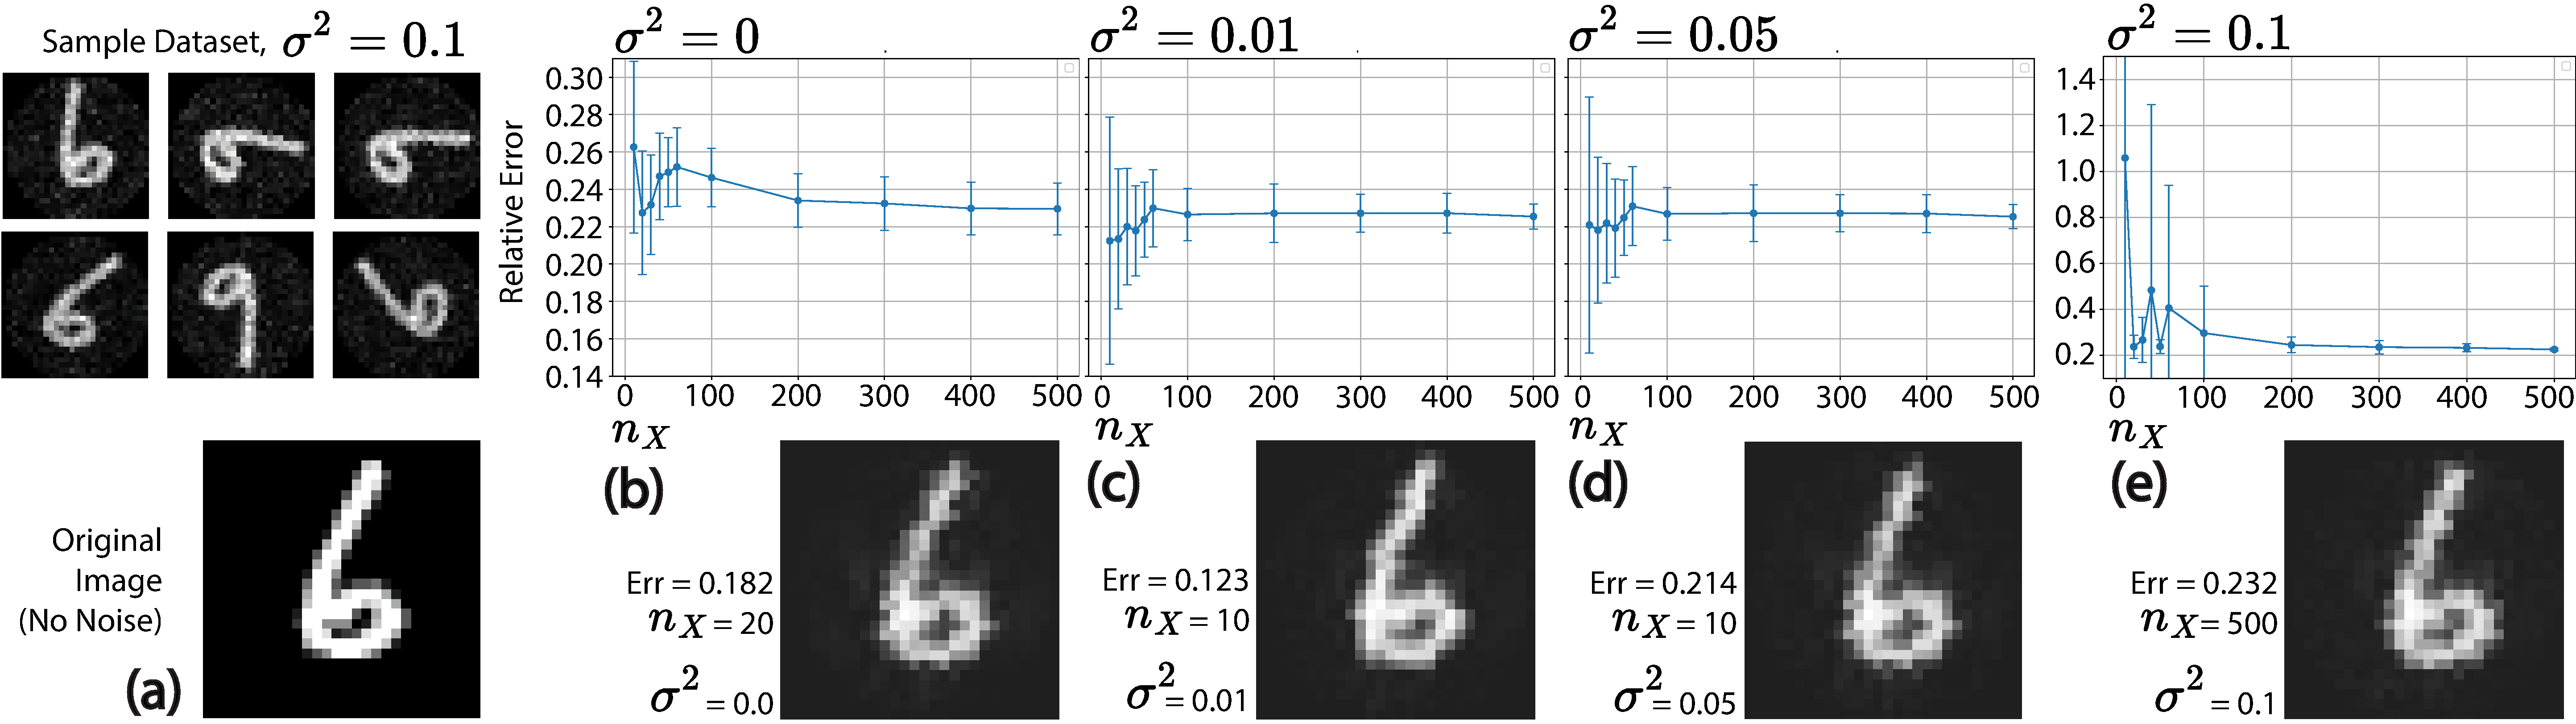
\includegraphics[width=\textwidth]{figs/mra_results.pdf}
    \caption[width=\textwidth]{(a) Dataset samples and original image used in MRA experiments for MNIST 6. (b-e) Relative error compares the similarity between the MRA reconstructed image and the original image used to generate the noisy rotated dataset for (b) $\sigma^2 = 0$ (c) $\sigma^2 = 0.01$, (d) $\sigma^2 = 0.05$, (e) $\sigma^2 = 0.1$. Sample reconstructions are shown below each result plot.}
    \label{fig:widecaption}

   \label{fig:mra-results}
\end{figure*}

To illustrate the computational and representational properties of our proposed selective disk bispectrum, we conduct a series of experiments testing \textit{speed}, \textit{invertibility}, and \textit{rotation invariance}. We compare against the full disk bispectrum proposed by \citep{zhao2014rotationally} and described in Eq. \ref{eq:disk_bispectrum}. Both the full and selective bispectra are computed using the disk harmonic coefficient library implemented by \citep{fast_dhcs_2023} on a MacBook Pro with an Apple M2 Max chip.

\subsection{Design of Tractability Experiments}

We consider square grayscale palm tree images of length \( L \in \{16 , 28, 56, 112\} \), each perturbed with Gaussian noise of standard deviation \( \sigma \in \{0, 0.01, 0.05, 0.1\} \). For each image, we compute both the full and selective disk bispectrum using the formulations in Eq.~\ref{eq:disk_bispectrum} (full) and Eq.~\ref{eq:selective_disk_bispectrum} (selective). We repeat these experiments for all digits of MNIST, and show results in the Appendix.

\textbf{Speed.} We compare the runtime of the forward and inverse bispectrum transforms across image sizes $L$ and noise levels $\sigma$. The full disk bispectrum is computationally expensive and impractical for many cases. In contrast, our \emph{selective disk bispectrum} enables efficient computation, making both encoding and reconstruction feasible even for larger images.

\textbf{Invertibility.} In the previous section, we prove that the selective disk bispectrum is \textit{complete}. Here, we visually confirm our theoretical results by constructing an image \( f \) from its bispectrum and measuring the relative reconstruction error $\varepsilon_{\text{rel}} = \frac{\left\lVert \hat{f} - f \right\rVert}{\left\lVert f \right\rVert}$, where \( \hat{f} \) is the image reconstruction obtained by applying the inverse map to the disk bispectrum coefficients. We observe in Fig. \ref{fig:tractability} that the selective bispectrum retains the essential information needed to accurately reconstruct the original image, demonstrating its practical completeness.

% \[
% \varepsilon_{\text{rel}} = \frac{\left\lVert \hat{f} - f \right\rVert}{\left\lVert f \right\rVert},
% \]

\textbf{Rotation Invariance.} We verify the invariance of the disk bispectrum to disk rotations. Given an image \( f \) and its rotated version \( f' \), we compute their respective bispectra \( b^{f} \) and \( b^{f'} \). Since the bispectrum is designed to be invariant to rotations, we expect $b^{f} = b^{f'}$. To quantify invariance, we compute the relative error between the two bispectra $\varepsilon_{\text{rel}} = \frac{\left\lVert b^{f} - b^{f'} \right\rVert}{\left\lVert b^{f} \right\rVert}$. Low error values across test conditions confirm that both the full and selective bispectra exhibit strong empirical rotation invariance, as shown in Fig.~\ref{fig:tractability}.
% \[
% \varepsilon_{\text{rel}} = \frac{\left\lVert b^{f} - b^{f'} \right\rVert}{\left\lVert b^{f} \right\rVert}.
% \]

\subsection{Results of Tractability Experiments}

We present the results of the tractability experiments. Full experimental results, including results on all MNIST images, are available in the Appendix.

\textbf{Speed.} The selective disk bispectrum offers a 3× speedup over the full bispectrum for \(16 \times 16\) images, and a 17,\!322× speedup for \(112 \times 112\) images. The inverse transform is equivalently fast for the full and selective bispectra, since the full bispectrum inversion utilizes only the subset of its coefficients included in the selective variant. Forward and inverse timing results are shown in Fig.~\ref{fig:tractability} for \(\sigma = 0\); run times are unaffected by noise level.

\textbf{Invariance.} Bispectrum invariance error decreases with higher image resolution, as shown in Fig.~\ref{fig:tractability}, and is as low as $3$ percent for $112\times112$ images. Invariance error is largely unaffected by noise level.

\textbf{Invertibility.} As shown in Fig.~\ref{fig:tractability}, the selective bispectrum accurately reconstructs the original image. This reconstruction accuracy is identical to the full bispectrum's. While reconstruction error increases slightly at lower tested resolutions, images are sufficiently reconstructed across all tested settings (see Appendix for reconstruction across bispectrum type, noise, and image resolution). Importantly, bispectrum inversions match the original image, up to a rotation. Since the bispectrum inversion reconstructs the original image up to a global rotation, reconstructions in Fig. ~\ref{fig:tractability} have been manually registered to match the orientation of the original image for clear comparison.
